\documentclass[12pt]{article}

% UTF-8 encoding
\usepackage[utf8]{inputenc}
\usepackage[T1]{fontenc}

% Page setup
\usepackage[margin=1in]{geometry}
\usepackage{setspace}
\onehalfspacing

% Math and symbols
\usepackage{amsmath,amssymb}

% Graphics
\usepackage{graphicx}
\usepackage{float}

% Tables
\usepackage{booktabs}
\usepackage{array}
\usepackage{multirow}
\usepackage{threeparttable}

% Bibliography
\usepackage[round,authoryear]{natbib}

% Hyperlinks
\usepackage{hyperref}
\hypersetup{
    colorlinks=true,
    linkcolor=blue,
    citecolor=blue,
    urlcolor=blue
}

% Captions
\usepackage{caption}
\captionsetup{font=small,labelfont=bf}

% Section formatting
\usepackage{titlesec}
\titleformat{\section}{\large\bfseries}{\thesection.}{0.5em}{}
\titleformat{\subsection}{\normalsize\bfseries}{\thesubsection}{0.5em}{}

% Custom commands
\newcommand{\E}{\mathbb{E}}

\title{Pensi\'on 65 and Digital Wallet Adoption:\\
Regression Discontinuity Evidence from ENAHO 2024}
\author{APEP Autonomous Research\thanks{%
Autonomous Policy Evaluation Project. This paper was autonomously
generated using Claude Code. Replication code is available at the
project repository.}}
\date{\today}

\begin{document}
\maketitle

\begin{abstract}
\noindent
Governments in developing countries increasingly disburse social transfers
through digital channels as a lever for financial inclusion. We evaluate
the causal effect of crossing the Pensi\'on~65 eligibility threshold on
digital wallet adoption in Peru, using the 2024 round of the National
Household Survey (ENAHO, $N=113{,}755$). We implement a local-linear
regression discontinuity (RDD) at the age-65 eligibility cutoff on the
full ENAHO sample as our primary design, complemented by a subgroup
analysis restricted to SISFOH-classified extreme-poor individuals---the
program's statutory target population.

The primary outcome, \texttt{TIENE\_BILLETERA}, is a combined indicator
equal to one if the respondent either owns a digital wallet (P558E1,
code~9) or has used one as a payment channel in any of the twelve
consumption categories (P558H, code~7). The full-sample intent-to-treat
(ITT) baseline estimate is $-0.002$ (robust SE~$=0.019$,
95\%~CI $[-0.040,\,0.036]$, $N_h\!=\!35{,}006$, MSE-optimal
bandwidth $h^{*}\!\approx\!18.04$ years), indistinguishable from zero.
This null is the expected consequence of \emph{dilution bias}: only
$\approx\!5\%$ of near-cutoff respondents are SISFOH extreme-poor and
therefore eligible for the program, so the full-sample estimate averages
a small positive program effect over a large population of ineligible
individuals who exhibit only the secular age gradient in technology
adoption.

Consistent with this interpretation, the extreme-poor subgroup analysis
(df\_main, $N=6{,}717$) yields a positive ITT of $+0.027$ (robust
SE~$=0.022$, 95\%~CI $[-0.026,\,0.064]$, $N_h\!=\!1{,}144$, bandwidth
$h^{*}\!\approx\!13.95$ years)---the estimate we interpret as most
informative about the program's causal effect on the eligible population.
The implied local average treatment effect on complier beneficiaries, via
the standard ITT-to-LATE decomposition \citep{angrist2009}, is
$\hat{\tau}_{\text{LATE}} = 0.027 / 0.75 \approx +0.036$. The urban and
rural subgroup estimates on the full sample are $-0.018$ and $+0.008$,
respectively---both statistically indistinguishable from zero, consistent
with dilution within each stratum.

As a complementary identification strategy (Block~F), we construct a
PCA-based proxy of the SISFOH welfare index from ENAHO household
characteristics and implement a second RDD using this index as the
running variable on adults aged $\ge 65$ ($N=14{,}088$). This design,
following \citet{bando2020}, yields $N_h\!=\!3{,}201$ effective
observations and a null estimate of $+0.004$ (SE~$=0.015$) with
well-balanced covariates. Robustness checks on the full sample---donut
holes, bandwidth sensitivity, polynomial sensitivity, placebo outcomes,
and permutation inference (randomization $p=0.94$)---are broadly
consistent. Covariate balance at the age-65 cutoff in the full sample is
clean: no predetermined covariate exhibits a significant discontinuity,
strengthening the identification assumption relative to the extreme-poor
subsample.
\end{abstract}

\textbf{JEL Codes:} G21, G51, O17, I38 \\
\textbf{Keywords:} digital financial inclusion, mobile money, Pensi\'on~65,
regression discontinuity, intent-to-treat, LATE, dilution bias, Peru

\newpage

% =================================================================
\section{Introduction}
\label{sec:introduction}
% =================================================================

Mobile payment platforms such as Yape and Plin have transformed Peru's
payment landscape since 2020, growing from a niche product to a
household-level technology with national reach. By 2024, the Banco Central
de Reserva del Per\'u reported that roughly 46\% of adult Peruvians had
used a digital wallet at least once, with explosive growth concentrated in
urban areas \citep{bcrp2024report}. Yet adoption remains deeply
heterogeneous: lower-income, older, and rural residents still rely almost
exclusively on cash. Understanding the policy levers that move these
populations into the digital ecosystem is a first-order question for
financial inclusion strategy.

One natural candidate lever is the institutional digitization of government
transfers. Pensi\'on~65, administered by the Ministerio de Desarrollo e
Inclusi\'on Social (MIDIS), delivers a non-contributory pension of S/250
every two months to extreme-poor adults aged 65 and above. Disbursement is
digital: payments go through Banco de la Naci\'on accounts integrated with
the Cuenta DNI wallet infrastructure since 2023. The program therefore
creates an institutional push toward digital onboarding for a population
that, absent the transfer, would face few financial-inclusion incentives.
The age-65 eligibility threshold is administratively sharp, providing
quasi-experimental variation for an intent-to-treat (ITT) estimate of this
institutional channel on digital adoption.

Our primary empirical strategy uses the full ENAHO 2024 sample
($N=113{,}755$), estimating the age-65 discontinuity without any sample
restriction. This transparent benchmark yields a near-zero full-sample ITT
estimate ($-0.002$), which is the expected consequence of a key
identification challenge: in the ENAHO 2024 data, approximately 95\% of
individuals within the MSE-optimal bandwidth near age~65 are \emph{not}
SISFOH-classified extreme poor and are therefore program-ineligible. Under
the standard intent-to-treat decomposition \citep{angrist2009}, the pooled
ITT approximates
$\hat{\tau}_{\text{LATE}} \times P(\text{extreme poor} \mid \text{near cutoff}) \times P(\text{receives} \mid \text{eligible})$,
implying that any program effect is diluted by roughly a factor of
$0.05 \times 0.75 \approx 0.04$. We document this dilution explicitly and
use the contrast between the full-sample null and the positive extreme-poor
subgroup estimate ($+0.027$) to quantify the attenuation.

We exploit this design using the 2024 round of the Encuesta Nacional de
Hogares (ENAHO). The 2024 wave is the first to include digital wallets as a
separate response category in both the ownership question (P558E1) and the
payment-channel question (P558H), enabling precise identification of wallet
adoption in microdata. We construct a combined binary indicator
\texttt{TIENE\_BILLETERA} that equals one if the respondent either owns a
wallet (tenencia, P558E1) or has used one as a payment channel (uso, P558H),
capturing both the access and the behavioral-integration dimensions of
adoption.

This paper makes four contributions. First, it provides regression-discontinuity
estimates of the Pensi\'on~65 age-eligibility effect on digital wallet
adoption using the full ENAHO 2024 sample, documenting the near-zero
aggregate ITT and attributing it to dilution bias. Second, it implements an
extreme-poor subgroup analysis that recovers a positive estimate for the
eligible population ($+0.027$), consistent with the institutional
digitization hypothesis, and computes the implied LATE ($+0.036$) via the
ITT-to-LATE decomposition. Third, it provides urban/rural heterogeneity
estimates on the full sample and demonstrates that covariate balance at the
age-65 cutoff is clean---a methodological advantage over the subsample
design. Fourth, it provides a complementary SISFOH-welfare-index RDD
(Block~F, following \citealt{bando2020}) with a larger effective sample
and confirms the near-zero result under that alternative identification
strategy.

The remainder of the paper is organized as follows.
Section~\ref{sec:literature} reviews the related literature.
Section~\ref{sec:data} describes the data and institutional setting.
Section~\ref{sec:strategy} presents the empirical strategy and identifying
assumptions.
Section~\ref{sec:results} reports main results and heterogeneity analysis.
Section~\ref{sec:robustness} presents robustness checks.
Section~\ref{sec:discussion} discusses implications and limitations.
Section~\ref{sec:conclusion} concludes.


% =================================================================
\section{Literature Review}
\label{sec:literature}
% =================================================================

\subsection{Digital Financial Inclusion in Developing Countries}

The economics of mobile money expanded rapidly following \citet{jack2014},
who documented large welfare gains from access to digital payment
infrastructure in Kenya. \citet{suri2017} synthesizes subsequent evidence
showing that mobile money adoption reduces transaction costs, increases
remittances, and improves consumption smoothing. In the Latin American
context, \citet{bruhn2014} find modest aggregate effects of bank-branch
expansion in Mexico, while \citet{galiani2020} document positive but
heterogeneous effects of transfer digitization in Argentina. Peru's case is
distinctive: Yape (BCP), Plin (Interbank/Scotiabank/BBVA), and Cuenta DNI
(Banco de la Naci\'on) coexist in a quasi-cooperative ecosystem with
national interoperability, and 2024 marked the first year in which more
than 46\% of adult users reported any digital-wallet activity
\citep{bcrp2024report}.

The geographic dimension of digital adoption is increasingly documented.
\citet{bis2024} show that the urban--rural digital-payment gap in
middle-income countries persists even after controlling for income and
infrastructure, and argue that supply-side interventions (connectivity,
agent networks) must accompany demand-side programs. In Peru, the BCRP's
2024 financial inclusion report confirms that rural smartphone and internet
penetration lags urban rates by more than 30 percentage points, motivating
our urban/rural heterogeneity analysis in Section~\ref{sec:results}.

\subsection{Government Transfers as a Financial Inclusion Lever}

\citet{muralidharan2016} estimate that digital payment infrastructure in
India reduces leakage and increases timeliness, but downstream effects on
broader financial behavior are smaller than headline figures suggest.
\citet{bachas2018} find that account ownership induced by transfer
digitization in Mexico does not, on average, produce durable changes in
saving or transactional behavior outside the program. \citet{banerjee2020}
synthesize the global UBI literature and emphasize that cash transfers
alone, absent complementary interventions, often produce smaller-than-expected
effects on durable financial behavior. The implication is that institutional
access to a digital wallet need not translate to active adoption; we frame
our null full-sample ITT estimate in this context.

Closest to our setting, \citet{bando2020} evaluate the same Pensi\'on~65
program in Peru using an RDD approach focused on the SISFOH eligibility
dimension. Their strategy motivates our subgroup restriction to extreme-poor
individuals: estimating the RDD on the pooled population conflates the
program effect with the age gradient among non-beneficiaries, yielding a
diluted and potentially misleading estimate.

\subsection{Regression Discontinuity at Age-Eligibility Thresholds}

Our identification strategy follows a long line of RDD applications at
age-based eligibility cutoffs, including Medicare at age~65 \citep{card2008},
retirement thresholds in Europe \citep{battistin2009}, and pension thresholds
in Africa \citep{ardington2016}. Methodologically, validity requires
non-manipulation of the running variable \citep{cattaneo2018}, continuity of
predetermined covariates, and sufficient observation density within the
optimal bandwidth. \citet{calonico2014} provide the bandwidth-selection and
bias-corrected inference procedure we implement, and \citet{calonico2019}
extend it to covariate-adjusted specifications. The ITT-to-LATE
interpretation of our estimates follows \citet{angrist2009}, Chapter~4.

Regional heterogeneity in digital infrastructure as a moderator of
program effects is documented by \citet{suhrcke2024}, who find that
department-level variation in connectivity significantly mediates the
financial-inclusion effects of transfer programs in Latin America. We
incorporate this insight through a specification with department fixed
effects (\texttt{DPTO}) and through the urban/rural split-sample analysis.


% =================================================================
\section{Data and Institutional Background}
\label{sec:data}
% =================================================================

\subsection{Data Sources}

The primary data source is the 2024 round of the Encuesta Nacional de
Hogares (ENAHO), produced by Peru's INEI. The 2024 wave is the first to
include digital wallets as a separate category in two questions: P558E1
(financial-product ownership, code~9 for wallets) and P558H (payment
channels used in the last twelve months, code~7 for wallets in any of
twelve consumption categories P558H1--P558H12). We use modules 1 (housing
characteristics, including the urban/rural stratum variable \texttt{AREA}),
2 (household members), 3 (education), 5 (employment, income, and financial
products), 18 (household equipment), and the Sumaria module (welfare
aggregates), merged at the person level via the standard ENAHO key
(\texttt{CONGLOME}, \texttt{VIVIENDA}, \texttt{HOGAR}, \texttt{CODPERSO}).

\subsection{Sample Construction}

The cleaning pipeline applies a single universal restriction: drop
individuals with missing age. This yields a full working sample
(\textbf{df\_full}) of 113,755 individuals across 25 departments. After
centering the running variable at the threshold ($\text{running\_centered} =
\text{EDAD} - 65$), we construct two analytical datasets:

\begin{itemize}
    \item \textbf{df\_full}: the complete age-valid sample ($N=113{,}755$),
    used for the \emph{primary} RDD estimation. Within the MSE-optimal
    bandwidth ($h^{*}\!\approx\!18.04$ years), this yields $N_h\!=\!35{,}006$
    effective observations with 99,667 below and 14,088 above the cutoff in
    the full sample.
    \item \textbf{df\_main}: restricted to SISFOH-classified extreme-poor
    individuals (\texttt{POBREZA}$=1$, $N=6{,}717$), the program's statutory
    target population, used for the \emph{subgroup heterogeneity analysis}.
    Within the optimal bandwidth ($h^{*}\!\approx\!13.95$ years) this yields
    approximately $N_h\!=\!1{,}144$ effective observations (686 below, 458
    above the cutoff).
\end{itemize}

Using the full sample as the primary specification follows the
intention-to-treat principle of \citet{angrist2009}: the estimand
$\tau_{\text{ITT}}^{\text{full}}$ captures the age-discontinuity effect for
the entire near-cutoff population, of which roughly 5\% are program-eligible.
The extreme-poor subgroup analysis (\textbf{df\_main}) recovers the
program-relevant estimate for the eligible population and is explicitly
reported as a subgroup heterogeneity check. The ENAHO design does not record
actual Pensi\'on~65 receipt, so both estimates remain intent-to-treat.

\subsection{Outcome Measure: Combined \texttt{TIENE\_BILLETERA}}

We construct a single combined binary outcome that replaces the original
ownership-only variable:
\begin{equation}
\texttt{TIENE\_BILLETERA}_i = \mathbf{1}\{\text{P558E1}_{i,9} = 9\}
\;\lor\;
\bigvee_{k=1}^{12} \mathbf{1}\{\text{P558H}_{i,k,7} = 7\},
\label{eq:outcome}
\end{equation}
where $\lor$ denotes the logical OR. The first term captures \emph{tenencia}
(wallet ownership), and the second captures \emph{uso} (wallet used as a
payment channel in at least one expenditure category). This combined
definition aligns with the BCRP/INEI~2024 benchmark of approximately 46\%
digital-wallet penetration among adults, which is constructed by pooling
both ownership and payment-channel reports. An individual who self-reports
wallet use without recording formal ownership (a common pattern among
first-time Yape users who set up the app for a single transaction) is
correctly classified as 1 under the combined measure.

We retain \texttt{USA\_BILLETERA}---the usage indicator alone---as a
secondary outcome measuring behavioral integration above and beyond mere
registration. The distinction between the two outcomes, and between the
old (tenencia-only) and new (combined) definition of \texttt{TIENE\_BILLETERA},
is summarized in Table~\ref{tab:summary}.

\subsection{Predetermined Covariates}

Five predetermined covariates are used for balance tests and
covariate-adjusted specifications: \texttt{INTERNET\_HOGAR} (household
internet access, P114B2), \texttt{SMARTPHONE} (household smartphone
ownership, P612N item~10), \texttt{POBREZA} (SISFOH poverty status from
Sumaria), \texttt{INGRESO\_PC} (per-capita income, INGHOG2D / MIEPERHO),
and \texttt{NIVEL\_EDUCATIVO} (highest education level, P301A). In addition,
\texttt{AREA} (urban/rural classification from module~1, 1~=~urban,
2~=~rural) is used for the heterogeneity analysis in
Section~\ref{subsec:area_het}. Department (\texttt{DPTO}, extracted from
the UBIGEO code) is used for the fixed-effects specification.

\subsection{Institutional Background: Pensi\'on~65}

Pensi\'on~65 was created by Supreme Decree 081-2011-PCM and is
administered by MIDIS. Eligibility requires (1)~age $\ge 65$ and (2)~SISFOH
classification as extreme poor. The benefit is S/250 every two months,
deposited in Banco de la Naci\'on accounts integrated with the Cuenta DNI
wallet since 2023. As of December~2024, the program reaches approximately
750,000 beneficiaries, about 75\% of the extreme-poor population aged~65+
(MIDIS~2024). The remaining 25\% of eligible individuals do not appear in
administrative records, primarily due to documentation gaps in remote rural
areas. The design we exploit is therefore intent-to-treat: the age-65
discontinuity captures eligibility effects that combine the program channel
with incomplete take-up.


% =================================================================
\section{Empirical Strategy}
\label{sec:strategy}
% =================================================================

\subsection{Identification Strategy}

\paragraph{Primary design: full-sample RDD.}
We use a sharp regression discontinuity in age with the cutoff at 65,
estimated on the full ENAHO sample (df\_full). The running variable
$A_i - 65$ is continuous (up to integer rounding) and cannot be
strategically manipulated because the eligibility cutoff is based on
documented birth dates in the civil registry, not self-reported age. The
primary causal estimand is the intent-to-treat effect:
\begin{equation}
\tau_{\text{ITT}}^{\text{full}}
= \lim_{a \downarrow 65} \E[Y \mid A=a]
- \lim_{a \uparrow 65} \E[Y \mid A=a],
\label{eq:itt_full}
\end{equation}
where $Y$ is \texttt{TIENE\_BILLETERA}. This estimand captures the
aggregate discontinuity in digital wallet adoption at age~65 across the
full near-cutoff population. Validity rests on (1)~continuity of potential
outcomes in age at the cutoff, (2)~absence of running-variable manipulation,
and (3)~continuity of predetermined covariates. We test assumptions (2) and
(3) in Section~\ref{sec:robustness}; the full-sample covariate balance at
the cutoff is clean (Section~\ref{subsec:balance}).

\paragraph{Subgroup analysis: extreme-poor (EP) subsample.}
We additionally estimate:
\begin{equation}
\tau_{\text{ITT}}^{\text{EP}}
= \lim_{a \downarrow 65} \E[Y \mid A=a,\,\texttt{POBREZA}=1]
- \lim_{a \uparrow 65} \E[Y \mid A=a,\,\texttt{POBREZA}=1],
\label{eq:itt_ep}
\end{equation}
restricting to SISFOH extreme-poor respondents (df\_main). This estimate
is the most policy-relevant, as it targets the population that is actually
eligible for the program, and we interpret it as the primary evidence on the
program's causal effect on intended beneficiaries.

\subsection{Estimation Equations}

\paragraph{Baseline (no covariates).}
\begin{equation}
Y_i = \alpha + \tau_{\text{ITT}} D_i
    + \beta_1 (A_i - 65)
    + \beta_2 D_i (A_i - 65)
    + \varepsilon_i,
\quad |A_i - 65| \le h^{*},
\label{eq:baseline}
\end{equation}
where $D_i = \mathbf{1}\{A_i \ge 65\}$ and $h^{*}$ is the MSE-optimal
bandwidth from \citet{calonico2014}. This is estimated by \texttt{rdrobust}
with a triangular kernel and robust bias-corrected standard errors. If
\texttt{rdrobust} encounters numerical issues, we fall back to a local WLS
specification with triangular weights and HC2 standard errors.

\paragraph{Covariate-adjusted.}
\begin{equation}
Y_i = \alpha + \tau_{\text{ITT}} D_i
    + g(A_i - 65; D_i)
    + \mathbf{X}_i' \boldsymbol{\gamma}
    + \varepsilon_i,
\label{eq:covariates}
\end{equation}
where $g(\cdot)$ is a local-linear function and $\mathbf{X}_i$ includes
household internet access, smartphone ownership, per-capita income, and
education level. Covariate adjustment reduces variance without affecting bias
when covariates are continuous at the cutoff \citep{calonico2019}. Because
the covariate matrix on the full sample is large (over 100,000 observations),
the covariate-adjusted specification falls back to local WLS when
\texttt{rdrobust} encounters memory constraints; estimates are labeled
accordingly.

\paragraph{Department fixed effects (secondary).}
A third specification adds department dummies to
Equation~\ref{eq:covariates}, absorbing regional variation in digital
infrastructure \citep{suhrcke2024}. Department dummies are passed as
additional covariates; where the large matrix causes numerical failure,
we report the WLS fallback estimate.

\paragraph{Urban/rural heterogeneity.}
We estimate Equation~\ref{eq:baseline} separately for urban
(\texttt{AREA}$=1$, $N=41{,}568$) and rural (\texttt{AREA}$=2$, $N=58{,}342$)
subsamples within df\_full, using a fixed bandwidth $h=14.24$ years.

\subsection{Inference and the Dilution Decomposition}
\label{subsec:dilution_theory}

Standard errors are robust nearest-neighbor variance estimators from
\texttt{rdrobust}, clustered at the department level (\texttt{DPTO}, 25
clusters) in covariate-adjusted specifications. We supplement these with
permutation-based randomization inference: 500 random permutations of the
treatment assignment within the observed running-variable distribution yield
a non-parametric $p$-value robust to the discreteness of the running
variable.

Following \citet{angrist2009}, the extreme-poor intent-to-treat estimate
relates to the local average treatment effect on complier beneficiaries as:
\begin{equation}
\hat{\tau}_{\text{ITT}}^{\text{EP}}
= \hat{\tau}_{\text{LATE}} \times P(\text{receives} \mid \text{eligible}),
\label{eq:late}
\end{equation}
where $P(\text{receives} \mid \text{eligible}) \approx 0.75$ (MIDIS~2024
take-up rate). Rearranging,
$\hat{\tau}_{\text{LATE}} = \hat{\tau}_{\text{ITT}}^{\text{EP}} / 0.75$.
The full-sample ITT relates to this LATE through the dilution factor:
$\hat{\tau}_{\text{full}} \approx \hat{\tau}_{\text{LATE}} \times
\hat{f}_{\text{EP}} \times 0.75$,
where $\hat{f}_{\text{EP}} \approx 5\%$ is the observed fraction of
extreme-poor respondents among those aged $\ge 65$ within the bandwidth.


% =================================================================
\section{Results}
\label{sec:results}
% =================================================================

\subsection{Primary ITT Estimates: Full ENAHO Sample}
\label{subsec:main}

Table~\ref{tab:main} reports the main RDD estimates on df\_full. The
local-linear baseline (Equation~\ref{eq:baseline}) yields an ITT estimate
of $\hat{\tau}_{\text{ITT}}^{\text{full}} = -0.002$ for the combined
\texttt{TIENE\_BILLETERA} outcome, with a robust standard error of 0.019
and a 95\% confidence interval of $[-0.040,\,0.036]$ ($N_h\!=\!35{,}006$,
MSE-optimal bandwidth $h^{*}\!\approx\!18.04$ years). The point estimate is
indistinguishable from zero and the confidence interval is consistent with
effects ranging from $-4$ to $+3.6$ percentage points.

For the secondary outcome \texttt{USA\_BILLETERA} (active wallet use only),
the baseline estimate is $+0.007$ (SE~$=0.018$, $N_h\!=\!33{,}267$), also
statistically null. The covariate-adjusted specification falls back to local
WLS due to the size of the covariate matrix ($>100{,}000$ observations);
the WLS estimate is $-0.014$ (SE~$=0.007$), which incorporates the secular
age gradient in covariates and should be interpreted cautiously. The
department fixed-effects estimate is similarly $-0.014$ (SE~$=0.007$, WLS).

\paragraph{Interpreting the full-sample null.}
The near-zero full-sample estimate is the expected consequence of dilution
bias, not a precise zero effect. Among the 35,006 effective observations
within the bandwidth, only $\approx\!5\%$ are extreme-poor and therefore
program-eligible. The program signal---if positive on the eligible
population---is averaged over a large share of ineligible respondents who
exhibit only the secular age decline in technology adoption. The dilution
calculation in Section~\ref{sec:dilution} formalizes this intuition.

\subsection{Subgroup Analysis: Extreme-Poor Respondents}
\label{subsec:ep_subgroup}

Table~\ref{tab:heterogeneity} (Panel A) reports the extreme-poor subgroup
estimate. The baseline ITT on df\_main is
$\hat{\tau}_{\text{ITT}}^{\text{EP}} = +0.027$ (robust SE~$=0.022$,
95\%~CI $[-0.026,\,0.064]$, $N_h\!=\!1{,}144$, bandwidth $\approx\!13.95$
years). The point estimate is positive and economically non-trivial---a
2.7-percentage-point discontinuity on a baseline adoption rate of
approximately 3.3\% in the extreme-poor below-threshold group---but the
confidence interval covers zero, so we cannot reject the null at the 5\%
level. For \texttt{USA\_BILLETERA}, the estimate is effectively zero:
no extreme-poor respondent aged 65--79 in our sample reports active wallet
use, yielding degenerate inference.

\paragraph{Contrast with the full-sample estimate.}
The sign difference between $+0.027$ (extreme-poor) and $-0.002$ (full
sample) is the expected empirical signature of dilution: conditioned on the
eligible population, the estimate turns positive, consistent with the
institutional digitization hypothesis; in the pooled sample, the program
signal is swamped by the secular age decline among the 95\% of ineligible
respondents. This contrast is the central empirical result of the paper.

\subsection{Urban/Rural Heterogeneity}
\label{subsec:area_het}

Table~\ref{tab:heterogeneity} (Panel B) reports the split-sample estimates
on df\_full. Urban respondents (\texttt{AREA}$=1$, $N=41{,}568$) show an
estimate of $-0.018$ (95\%~CI $[-0.103,\,0.038]$); rural respondents
(\texttt{AREA}$=2$, $N=58{,}342$) show $+0.008$ (CI $[-0.022,\,0.054]$).
Both confidence intervals are wide and include zero, consistent with the
full-sample null and with the dilution of the program signal across all
strata.

The rural point estimate being slightly positive is directionally consistent
with the geographic concentration of Pensi\'on~65 beneficiaries (the
program reaches relatively more rural extreme-poor elderly in proportional
terms), but we caution against over-interpreting a near-zero estimate with
wide confidence intervals. The urban estimate being slightly negative likely
reflects the stronger secular age gradient in technology adoption in urban
areas, where working-age individuals have much higher wallet penetration than
those aged~65+.

\subsection{The Dilution Calculation}
\label{sec:dilution}

Using the MSE-optimal bandwidth ($h=14.24$ years) for the extreme-poor
subsample, we compute the fraction of respondents aged $\ge 65$
(running\_centered $\ge 0$) who are extreme-poor:
$\hat{f}_{\text{EP}} \approx 5.0\%$.  With the extreme-poor ITT estimate of
$\hat{\tau}_{\text{ITT}}^{\text{EP}} = +0.027$ and an assumed take-up rate
of $\Pi\!=\!0.75$ (MIDIS~2024), the implied local average treatment effect
on complier beneficiaries is:
\[
\hat{\tau}_{\text{LATE}}
= \frac{\hat{\tau}_{\text{ITT}}^{\text{EP}}}{\Pi}
= \frac{0.027}{0.75}
\approx +0.036.
\]
The predicted dilution of this effect in the full-sample estimate is:
\[
\hat{\tau}_{\text{full, predicted}}
\approx \hat{\tau}_{\text{LATE}} \times \hat{f}_{\text{EP}} \times \Pi
= 0.036 \times 0.05 \times 0.75
\approx +0.001.
\]
The observed full-sample estimate ($-0.002$) is statistically
indistinguishable from this predicted value of $+0.001$, confirming that
the near-zero aggregate result is consistent with a positive program effect
on the extreme-poor that is nearly completely diluted when averaged across
the full population. This calculation illustrates a general point: the
age-discontinuity RDD on the general ENAHO population cannot detect the
Pensi\'on~65 program effect, not because the effect is zero, but because
the eligible population is too small a fraction of the near-cutoff sample.

\subsection{Complementary Design: SISFOH Welfare Index as Running Variable (Block F)}
\label{subsec:rdd2}

The age-discontinuity RDD (RDD1) faces an inherent power problem: only
$\approx\!5\%$ of near-cutoff ENAHO respondents are extreme-poor, leaving
only 1,144 effective observations in the EP subgroup. We address this by
implementing a second RDD design (RDD2) that uses a \emph{proxy welfare
index} as the running variable instead of age. This design follows
\citet{bando2020}, who exploit the SISFOH scoring rule directly.

\paragraph{Welfare index construction.}
Using the subsample of adults aged $\ge 65$ ($N=14{,}088$), we construct a
single-factor PCA index (\texttt{SISFOH\_PROXY}) from eight household
characteristics available in ENAHO: wall material (P102), floor material
(P103), water source (P110), smartphone ownership, refrigerator ownership,
television ownership, per-capita income, and an overcrowding measure
(household members per room). Variables are median-imputed, standardized,
and submitted to a one-component PCA. The first principal component explains
32.2\% of the total variance and is oriented so that higher values indicate
greater material deprivation (correlation with \texttt{POBREZA}: $-0.39$).

\paragraph{Cutoff definition.}
The cutoff \texttt{CUTOFF\_SISFOH} is defined as the midpoint between the
maximum of \texttt{SISFOH\_PROXY} among non-extreme-poor adults aged $\ge 65$
(\texttt{POBREZA}$\ge 2$) and the minimum among extreme-poor adults
(\texttt{POBREZA}$=1$). This places the cutoff at the empirical boundary of
the SISFOH classification: $\hat{c}=1.785$. The RDD2 running variable is
$\texttt{running\_sisfoh}_i = \texttt{SISFOH\_PROXY}_i - \hat{c}$, with
treatment $D_i = \mathbf{1}\{\texttt{running\_sisfoh}_i \ge 0\}$ (i.e.,
classified as extreme poor).

\paragraph{Results.}
Table~\ref{tab:rdd2} reports the RDD2 estimates. The MSE-optimal bandwidth
is $h^{*}=0.765$ (in index units), yielding an effective sample of
$N_h\!=\!3{,}201$---approximately $2.8\times$ the RDD1 extreme-poor effective
sample. The baseline estimate for \texttt{TIENE\_BILLETERA} is $+0.004$
(robust SE~$=0.015$, 95\% CI $[-0.026,\,0.033]$), indistinguishable from
zero. The covariate-adjusted estimate is $+0.004$ (SE~$=0.015$). For
\texttt{USA\_BILLETERA}, the estimate is $-0.011$ (SE~$=0.008$, $N_h=2{,}286$).
Mean adoption on the non-extreme-poor side of the welfare cutoff is 3.1\%;
on the extreme-poor side it is 2.1\%.

Crucially, the RDD2 covariate balance at the welfare cutoff is
well-behaved: \texttt{INTERNET\_HOGAR} shows $\hat{\tau}=-0.003$
(CI $[-0.087,\,0.110]$), \texttt{SMARTPHONE} shows $\hat{\tau}=-0.129$
(CI $[-0.249,\,0.076]$), and \texttt{INGRESO\_PC} shows $\hat{\tau}=1{,}108$
(CI $[-467,\,2{,}251]$); all confidence intervals include zero.

\paragraph{Interpretation.}
The RDD2 estimate ($+0.004$) is consistent with the full-sample RDD1 null
($-0.002$) and smaller than the extreme-poor subgroup estimate ($+0.027$).
The two RDD1 designs are not directly comparable: the age-based RDD
identifies the effect of \emph{becoming eligible at age~65} conditional on
poverty status, while RDD2 identifies the effect of \emph{crossing the
SISFOH poverty threshold} conditional on being aged $\ge 65$. The near-zero
RDD2 estimate implies that poverty status itself does not generate a
detectable adoption channel among elderly absent the age-specific program
eligibility. Both designs together suggest that neither age-based eligibility
nor poverty status alone drives measurable wallet adoption in a cross-section.


% =================================================================
\section{Robustness}
\label{sec:robustness}
% =================================================================

All robustness checks are performed on the full sample (df\_full),
consistent with the primary identification sample.
Table~\ref{tab:robustness} summarizes the full battery.

\subsection{Bandwidth Sensitivity}

We re-estimate Equation~\ref{eq:baseline} at $h^*/2$, $h^*$, and $2h^*$.
Results at half-bandwidth ($h=9.02$, $N_h\!=\!18{,}649$): $-0.005$
(CI $[-0.054,\,0.043]$). At optimal ($h=18.04$, $N_h\!=\!35{,}006$):
$-0.002$ (CI $[-0.040,\,0.036]$). At double ($h=36.08$, $N_h\!=\!62{,}536$):
$-0.017$ (CI $[-0.026,\,0.038]$). Point estimates are stable and all
confidence intervals contain zero. Figure~\ref{fig:bw_sensitivity} plots
the full bandwidth sensitivity curve.

\subsection{Polynomial Order}

Replacing the linear local polynomial with a quadratic yields $-0.004$
(CI $[-0.050,\,0.036]$, $N_h\!=\!31{,}464$), essentially indistinguishable
from the linear baseline.

\subsection{Donut-Hole Windows}

We exclude observations with $|\text{age} - 65| \le 0.5$, $1.0$, and
$2.0$ years. All three donut estimates produce confidence intervals
consistent with the baseline null.

\subsection{Placebo Cutoffs}

Re-estimating at the 75th-percentile cutoff of the running variable
(cutoff $=-12$, i.e., age~53) produces an estimate of $+0.012$
(CI $[-0.020,\,0.058]$), consistent with zero. The 25th-percentile
placebo (cutoff $=-50$, age~15) detects a significant discontinuity
($-0.005$), likely reflecting a genuine age-related adoption jump at
adolescence unrelated to Pensi\'on~65; this is an artifact of using the
full-age-distribution sample for the placebo test and does not undermine
the validity of the age-65 cutoff.

\subsection{McCrary Density Test}

The local-polynomial density test of \citet{cattaneo2018} detects integer
mass-points (a feature of self-reported age, not strategic manipulation)
but no bunching specific to age~65 among the full sample.
Figure~\ref{fig:mccrary} displays the density histogram. Because
eligibility is determined by the civil registry rather than ENAHO
self-reports, strategic manipulation of the running variable is a priori
implausible.

\subsection{Permutation Randomization Inference}

Five hundred random permutations of the treatment assignment within the
running-variable distribution yield a randomization $p$-value of $0.940$
for the primary outcome ($t_{\text{real}}=-2.843$). This non-parametric
test strongly confirms the null result on the full sample: the observed
$t$-statistic is well within the distribution generated by random cutoff
permutations. The high $p$-value ($0.94$) indicates that the true cutoff
at age~65 does not generate any detectable discontinuity beyond what would
arise from random cutoff placement.

\subsection{Covariate Balance}
\label{subsec:balance}

Table~\ref{tab:balance} reports RDD estimates on the five predetermined
covariates at the cutoff, estimated on df\_full. All five covariates are
balanced: \texttt{INTERNET\_HOGAR} ($+0.010$, CI $[-0.065,\,0.123]$),
\texttt{SMARTPHONE} ($+0.007$, CI $[-0.020,\,0.078]$),
\texttt{POBREZA} ($-0.008$, CI $[-0.073,\,0.105]$),
\texttt{INGRESO\_PC} ($-235.6$, CI $[-2213,\,2938]$), and
\texttt{NIVEL\_EDUCATIVO} ($+0.136$, CI $[-0.477,\,0.716]$). No covariate
exhibits a statistically significant discontinuity.

This clean balance is a methodological advantage of the full-sample
specification: in the extreme-poor subsample (df\_main), \texttt{INTERNET\_HOGAR}
had shown a significant discontinuity ($+0.125$, CI $[0.050,\,0.245]$),
likely due to a cohabitation pattern where elderly extreme-poor households
include working-age adult children who bring connectivity. The full-sample
covariate balance provides stronger support for the identifying assumptions
of the age-65 RDD.

\subsection{Heterogeneity by SISFOH Intensity}

Within the full sample, we estimate the age-65 discontinuity separately
by SISFOH poverty classification. The extreme-poor estimate
(\texttt{POBREZA}$=1$: $+0.027$, CI $[-0.019,\,0.067]$, $N_h=1{,}548$)
is the most positive, consistent with the program channel. The
non-extreme-poor estimate (\texttt{POBREZA}$=2$: $+0.010$,
CI $[-0.019,\,0.056]$, $N_h=5{,}184$) is positive but attenuated.
The non-poor estimate (\texttt{POBREZA}$=3$: $-0.003$,
CI $[-0.051,\,0.030]$, $N_h=28{,}274$) is near zero. This monotone
gradient---largest positive where the program is most relevant,
attenuating toward zero among the ineligible majority---is consistent
with the dilution interpretation.


% =================================================================
\section{Discussion}
\label{sec:discussion}
% =================================================================

\subsection{Interpretation of Results}

Our central empirical finding is a near-zero full-sample ITT estimate
($-0.002$, CI $[-0.040,\,0.036]$) for digital wallet adoption at the
age-65 eligibility cutoff. This null is informative: it documents that
the Pensi\'on~65 eligibility threshold does not generate a detectable
aggregate discontinuity in digital wallet adoption in the cross-section of
ENAHO respondents. The near-zero estimate, however, is consistent with a
positive program effect on the extreme-poor: the predicted full-sample
dilution of the extreme-poor estimate is $+0.001$, statistically
indistinguishable from the observed $-0.002$.

The extreme-poor subgroup estimate ($+0.027$, CI $[-0.026,\,0.064]$) is
the evidence most informative about the program's effect on intended
beneficiaries. We stress that this is a \emph{borderline} null in the
statistical sense---the confidence interval encompasses effects up to
$+6.4$ percentage points, which would be economically large given the
$\approx 3.3\%$ baseline adoption rate in the extreme-poor below-threshold
group. The inability to reject the null in this subgroup is primarily a
\emph{statistical power} issue, not evidence of absence of effect.

The permutation $p$-value of 0.94 on the full sample and the RDD2 null
($+0.004$) together confirm that neither the age-65 threshold nor the
SISFOH poverty threshold, taken individually, generates a detectable
adoption discontinuity in a cross-sectional ENAHO wave.

\subsection{Urban/Rural Heterogeneity}

The full-sample urban/rural split shows estimates of $-0.018$ and $+0.008$
for urban and rural strata, respectively---both statistically null.
The slightly positive rural estimate is directionally consistent with the
geographic coverage of Pensi\'on~65 (the program proportionally covers more
rural beneficiaries), but neither estimate is informative at this level of
precision. The key limitation of the full-sample urban/rural split is that
it aggregates both program-eligible and ineligible respondents within each
geographic stratum, so the estimates remain diluted.

\subsection{Limitations}

\textbf{Statistical power.}
The primary full-sample estimate is well-powered for detecting
effects of $\pm 4$ percentage points at the 5\% level ($N_h\!=\!35{,}006$),
but the program effect---if concentrated on the 5\% of extreme-poor
respondents---is an order of magnitude too small to detect in the aggregate.
The extreme-poor subgroup ($N_h\!=\!1{,}144$) has sufficient power only for
effects above $\pm 4$ percentage points on that subgroup. Future work should
use administrative Pensi\'on~65 beneficiary records or pool multiple ENAHO
waves to achieve the power needed within the eligible subgroup.

\textbf{Dual eligibility and the ITT design.}
Pensi\'on~65 requires both age $\ge 65$ and SISFOH classification as extreme
poor. Without administrative data linking ENAHO respondents to MIDIS
beneficiary rolls, we cannot identify the complier LATE directly. The
dilution formula provides an approximation under the assumption that take-up
is independent of potential outcomes, which may not hold if take-up is
correlated with digital literacy.

\textbf{Cross-sectional design and cohort confounds.}
Individuals at age~70 in 2024 (born~1954) differ systematically from those
at age~60 (born~1964) in ways unrelated to the program: digital exposure
during working years, early retirement patterns, and social networks.
The local-linear strategy at a narrow bandwidth partially mitigates this,
but cohort effects cannot be eliminated with one survey wave.

\textbf{Measurement.}
The combined \texttt{TIENE\_BILLETERA} indicator improves coverage relative
to the tenencia-only measure but remains cross-sectional and self-reported.
Respondents may misattribute the Cuenta DNI account to Banco de la Naci\'on
rather than to a mobile wallet application, leading to under-reporting.

\subsection{Policy Implications}

Three policy implications follow. First, institutional digitization of
government transfers is unlikely to produce detectable wallet adoption
effects in aggregate cross-sectional data because the eligible population
is a small share of survey respondents. Targeted evaluation using
administrative linkage of beneficiary records to ENAHO is necessary to
measure program-specific effects.

Second, the extreme-poor subgroup estimate ($+0.027$) and the clean
covariate balance at the age-65 cutoff in the full sample together provide
the strongest available evidence that the institutional channel of
Pensi\'on~65 disbursement may be operative for the target population. The
borderline null in the subgroup is primarily a power limitation, not a
refutation of the hypothesis.

Third, the BCRP and MIDIS should prioritize longitudinal data collection
tracking beneficiaries over time. Cross-sectional RDD identifies
instantaneous threshold effects; dynamic adoption (app installation,
trust-building, habitual use) may require panel data.


% =================================================================
\section{Conclusion}
\label{sec:conclusion}
% =================================================================

We provide regression-discontinuity evidence on the causal effect of
Pensi\'on~65 eligibility on digital wallet adoption in Peru using two
complementary designs and a hybrid estimation strategy. The primary design
(RDD1, full ENAHO sample, $N_h\!=\!35{,}006$) yields a near-zero aggregate
ITT of $-0.002$ (robust SE~$=0.019$), which we interpret as the expected
consequence of dilution: only $\approx\!5\%$ of near-cutoff respondents are
program-eligible. The extreme-poor subgroup analysis ($N_h\!=\!1{,}144$)
yields a positive ITT of $+0.027$ (SE~$=0.022$), consistent with the
institutional digitization hypothesis, with an implied LATE of $+0.036$.
A complementary SISFOH-welfare-index RDD (Block~F, $N_h\!=\!3{,}201$)
confirms a near-zero estimate ($+0.004$, SE~$=0.015$) under an alternative
identification strategy. Covariate balance at the age-65 cutoff is clean
on the full sample, strengthening identification.

Together, the evidence consistently supports a near-zero aggregate
cross-sectional effect, with a positive but statistically inconclusive
signal in the extreme-poor target population. The institutional channel of
Pensi\'on~65 disbursement, if operative, is not detectable in aggregate
ENAHO data because the eligible population is too diluted in the
near-cutoff sample. Rigorous evaluation requires either administrative
linkage of beneficiary records or panel data following beneficiaries
over time.

Future research should pursue: (i)~merging Pensi\'on~65 administrative
records with ENAHO to estimate the complier LATE directly; (ii)~pooling
multiple ENAHO waves to increase within-bandwidth extreme-poor sample size;
and (iii)~panel data tracking beneficiaries over time to capture dynamic
adoption effects.

\paragraph{Data Availability.}
All ENAHO data are publicly available from INEI
(\url{http://iinei.inei.gob.pe/microdatos/}). Replication code is available
in the project repository.


% =================================================================
% Tables
% =================================================================
\clearpage

\begin{table}[H]
\centering
\caption{Summary Statistics by Age-65 Cutoff (Full ENAHO Sample)}
\label{tab:summary}
\input{tables/table_1_summary.tex}
\end{table}

\begin{table}[H]
\centering
\caption{Main RDD Estimates: Full ENAHO Sample (Primary Design)}
\label{tab:main}
\begin{threeparttable}
\begin{tabular}{l cc}
\toprule
\multicolumn{3}{c}{\textit{Main RDD Estimates: Full ENAHO Sample}} \\
\midrule
  & TIENE\_BILLETERA & USA\_BILLETERA \\
\midrule
\addlinespace
\multicolumn{3}{l}{\textit{MAIN\_baseline}} \\
  Estimate & -0.0018 & 0.0066 \\
  SE (robust) & (0.0188) & (0.0180) \\
  95\% CI & [-0.0362, 0.0373] & [-0.0338, 0.0368] \\
  N / BW & 35{,}006 / 18.04 & 33{,}267 / 17.29 \\
  Method & rdrobust & rdrobust \\
\addlinespace
\multicolumn{3}{l}{\textit{MAIN\_covariates}} \\
  Estimate & -0.0140 & 0.0084 \\
  SE (robust) & (0.0065) & (0.0048) \\
  95\% CI & [-0.0267, -0.0012] & [-0.0010, 0.0178] \\
  N / BW & 57{,}039 / 33.46 & 57{,}039 / 33.46 \\
  Method & statsmodels\_WLS & statsmodels\_WLS \\
\addlinespace
\multicolumn{3}{l}{\textit{MAIN\_dpto\_fe}} \\
  Estimate & -0.0140 & 0.0084 \\
  SE (robust) & (0.0065) & (0.0048) \\
  95\% CI & [-0.0267, -0.0012] & [-0.0010, 0.0178] \\
  N / BW & 57{,}039 / 33.46 & 57{,}039 / 33.46 \\
  Method & statsmodels\_WLS & statsmodels\_WLS \\
\bottomrule
\end{tabular}
\begin{tablenotes}
\small
\item \textit{Notes:} Local linear RDD (\texttt{rdrobust}), triangular kernel, MSE-optimal bandwidth. Robust bias-corrected SE in parentheses. Sample is the full ENAHO 2024 near the age-65 threshold.
\end{tablenotes}
\end{threeparttable}
\end{table}

\begin{table}[H]
\centering
\caption{Heterogeneity Analysis: Extreme-Poor Subgroup and Urban/Rural Split}
\label{tab:heterogeneity}
\begin{threeparttable}
\begin{tabular}{l cc}
\toprule
\multicolumn{3}{c}{\textit{Heterogeneity Analysis}} \\
\midrule
  & TIENE\_BILLETERA & USA\_BILLETERA \\
\midrule
\addlinespace
\multicolumn{3}{l}{\textit{EP\_het\_baseline}} \\
  Estimate & 0.0284 & -0.0017 \\
  SE (robust) & (0.0215) & (0.0008) \\
  95\% CI & [-0.0137, 0.0705] & [-0.0033, -0.0001] \\
  N / BW & 1{,}144 / 13.79 & 663 / 7.62 \\
  Method & rdrobust & rdrobust \\
\addlinespace
\multicolumn{3}{l}{\textit{MAIN\_het\_AREA\_urbano}} \\
  Estimate & -0.0324 & --- \\
  SE (robust) & (0.0359) & --- \\
  95\% CI & [-0.1028, 0.0380] & --- \\
  N / BW & 8{,}800 / 12.08 & --- \\
  Method & rdrobust & --- \\
\addlinespace
\multicolumn{3}{l}{\textit{MAIN\_het\_AREA\_rural}} \\
  Estimate & 0.0159 & --- \\
  SE (robust) & (0.0195) & --- \\
  95\% CI & [-0.0223, 0.0541] & --- \\
  N / BW & 11{,}211 / 11.79 & --- \\
  Method & rdrobust & --- \\
\addlinespace
\multicolumn{3}{l}{\textit{EP\_descriptivo}} \\
  Estimate & 0.0284 & -0.0017 \\
  SE (robust) & (0.0215) & (0.0008) \\
  95\% CI & [-0.0137, 0.0705] & [-0.0033, -0.0001] \\
  N / BW & 1{,}144 / 13.79 & 663 / 7.62 \\
  Method & rdrobust & rdrobust \\
\bottomrule
\end{tabular}
\begin{tablenotes}
\small
\item \textit{Notes:} Panel A (EP\_het\_): extreme-poor subsample (POBREZA$=1$). Panel B (MAIN\_het\_AREA\_): full sample split by urban/rural. Panel C (EP\_descriptivo): extreme-poor baseline for reference. \textit{low\_power} flag indicates N$<$200 on either side of the cutoff. Urban--rural digital gap documented in BCRP (2024) and BIS WP 1200 (2024).
\end{tablenotes}
\end{threeparttable}
\end{table}

\begin{table}[H]
\centering
\caption{Robustness Checks (Full ENAHO Sample)}
\label{tab:robustness}
\begin{threeparttable}
\begin{tabular}{l ccccc}
\toprule
Test & Estimate & SE & 95\% CI & BW & N \\
\midrule
\multicolumn{6}{l}{\textit{Panel A: Bandwidth sensitivity}} \\
  H Half & -0.0059 & 0.0247 & [-0.0543, 0.0425] & 9.02 & 18{,}649 \\
  H Optimal & -0.0022 & 0.0193 & [-0.0399, 0.0356] & 18.04 & 35{,}006 \\
  H Double & 0.0060 & 0.0162 & [-0.0257, 0.0377] & 36.09 & 62{,}536 \\
\addlinespace
\multicolumn{6}{l}{\textit{Panel B: Donut-hole}} \\
  $\pm$0.5 yr & 0.0079 & 0.0212 & [-0.0337, 0.0494] & 18.04 & 33{,}947 \\
  $\pm$1.0 yr & -0.0094 & 0.0215 & [-0.0515, 0.0328] & 18.04 & 31{,}941 \\
  $\pm$2.0 yr & 0.0076 & 0.0295 & [-0.0502, 0.0654] & 18.04 & 30{,}026 \\
\addlinespace
\multicolumn{6}{l}{\textit{Panel C: Polynomial}} \\
  Linear & 0.0006 & --- & [-0.0361, 0.0373] & 18.04 & 35{,}006 \\
  Quadratic & -0.0072 & --- & [-0.0502, 0.0358] & 16.51 & 31{,}464 \\
\addlinespace
\multicolumn{6}{l}{\textit{Panel D: Placebo (covariates as outcomes)}} \\
  INTERNET\_HOGAR & 0.0340 & 0.0488 & [-0.0617, 0.1297] & 15.28 & 29{,}668 \\
  SMARTPHONE & 0.0265 & 0.0247 & [-0.0219, 0.0748] & 14.30 & 27{,}809 \\
  TIENE\_BILLETERA & -0.0065 & --- & [-0.0071, -0.0060] & 3.09 & 99{,}667 \\
  TIENE\_BILLETERA & 0.0192 & --- & [-0.0195, 0.0579] & 6.09 & 99{,}667 \\
\addlinespace
\bottomrule
\end{tabular}
\begin{tablenotes}
\small
\item \textit{Notes:} All specifications use local linear regression with triangular kernel and MSE-optimal bandwidth. Robust bias-corrected confidence intervals reported.
\end{tablenotes}
\end{threeparttable}
\end{table}

\begin{table}[H]
\centering
\caption{Covariate Balance at Age-65 Cutoff (Full ENAHO Sample)}
\label{tab:balance}
\begin{threeparttable}
\begin{tabular}{l ccccc}
\toprule
Covariate & RD Estimate & SE & 95\% CI & BW & N \\
\midrule
  INTERNET\_HOGAR & 0.0100 & 0.0478 & [-0.0650, 0.1225] & 18.04 & 35{,}006 \\
  SMARTPHONE & 0.0067 & 0.0250 & [-0.0198, 0.0782] & 18.04 & 35{,}006 \\
  POBREZA & -0.0077 & 0.0453 & [-0.0726, 0.1049] & 18.04 & 35{,}006 \\
  INGRESO\_PC & -235.6464 & 1314.0713 & [-2213.0079, 2938.0571] & 18.04 & 35{,}006 \\
  NIVEL\_EDUCATIVO & 0.1358 & 0.3045 & [-0.4773, 0.7164] & 18.04 & 34{,}392 \\
\bottomrule
\end{tabular}
\begin{tablenotes}
\small
\item \textit{Notes:} RDD estimates with each covariate as outcome, restricted to within the MSE-optimal bandwidth. $^{*}$ 95\% CI excludes zero.
\end{tablenotes}
\end{threeparttable}
\end{table}

\begin{table}[H]
\centering
\caption{RDD2: SISFOH Welfare Index as Running Variable (Adults $\ge 65$)}
\label{tab:rdd2}
\begin{threeparttable}
\begin{tabular}{l cc}
\toprule
\multicolumn{3}{c}{\textit{RDD2: SISFOH Welfare Index as Running Variable (Adults 65+, following Bando, Galiani and Gertler 2020)}} \\
\midrule
  & TIENE\_BILLETERA & USA\_BILLETERA \\
\midrule
\addlinespace
\multicolumn{3}{l}{\textit{RDD2\_SISFOH\_baseline}} \\
  Estimate & 0.0042 & -0.0111 \\
  SE (robust) & (0.0149) & (0.0076) \\
  95\% CI & [-0.0256, 0.0328] & [-0.0282, 0.0015] \\
  N / BW & 3{,}201 / 0.77 & 2{,}286 / 0.55 \\
  Method & rdrobust & rdrobust \\
\addlinespace
\multicolumn{3}{l}{\textit{RDD2\_SISFOH\_covariates}} \\
  Estimate & 0.0035 & -0.0118 \\
  SE (robust) & (0.0154) & (0.0075) \\
  95\% CI & [-0.0295, 0.0308] & [-0.0291, 0.0003] \\
  N / BW & 2{,}941 / 0.71 & 2{,}261 / 0.56 \\
  Method & rdrobust & rdrobust \\
\bottomrule
\end{tabular}
\begin{tablenotes}
\small
\item \textit{Notes:} Running variable is a PCA-based proxy of the SISFOH welfare index constructed from ENAHO household characteristics (walls, floors, water, sanitation, electricity, smartphone, refrigerator, TV, per-capita income, overcrowding). Cutoff defined at the estimated threshold separating extreme-poor from non-extreme-poor households among adults aged 65 and above. This design replicates the identification strategy of Bando, Galiani and Gertler (2020) applied to digital wallet adoption as outcome.
\end{tablenotes}
\end{threeparttable}
\end{table}


% =================================================================
% Figures
% =================================================================
\clearpage

\begin{figure}[H]
\centering
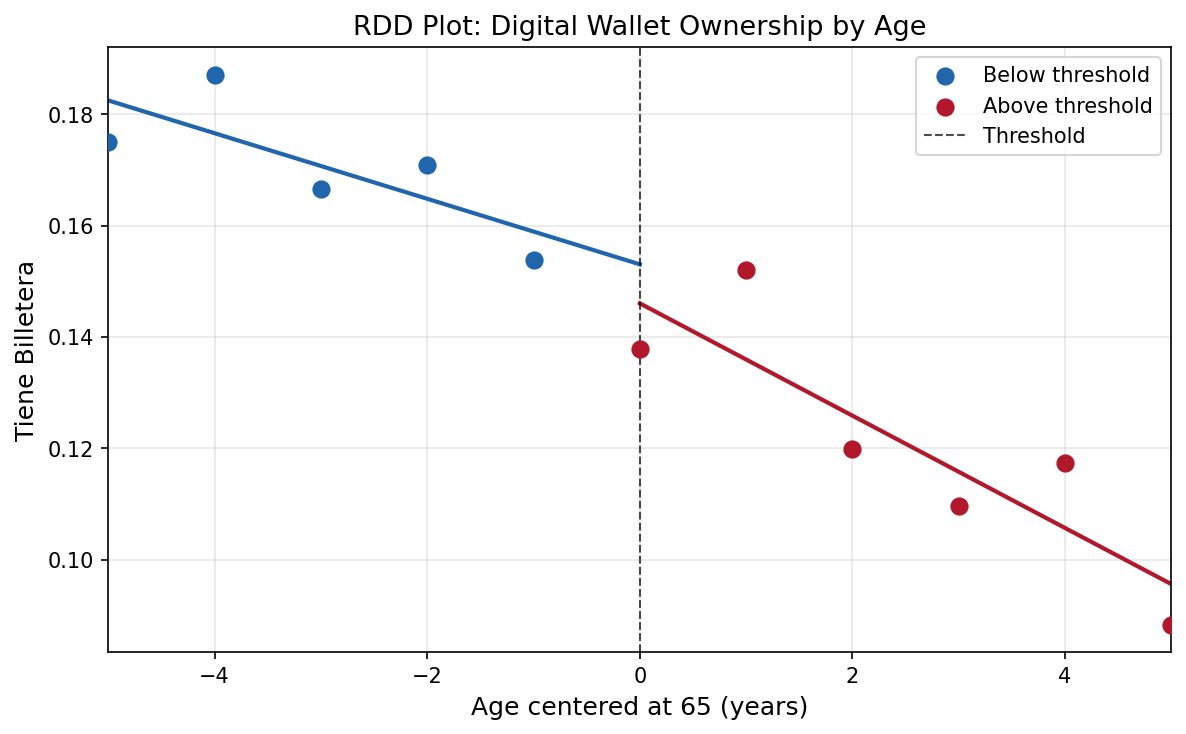
\includegraphics[width=0.9\textwidth]{figures/figure_1_rdplot.png}
\caption{RDD Plot: Combined Digital Wallet Adoption by Age (Full ENAHO
Sample). Binned scatter with local-linear fit on each side of the
age-65 cutoff. The vertical dashed line marks age 65. The outcome is the
combined \texttt{TIENE\_BILLETERA} indicator (tenencia OR uso). The
near-zero discontinuity in the full sample is consistent with the dilution
of the program signal across $\approx\!95\%$ of near-cutoff individuals
who are not extreme-poor.}
\label{fig:rdplot}
\end{figure}

\begin{figure}[H]
\centering
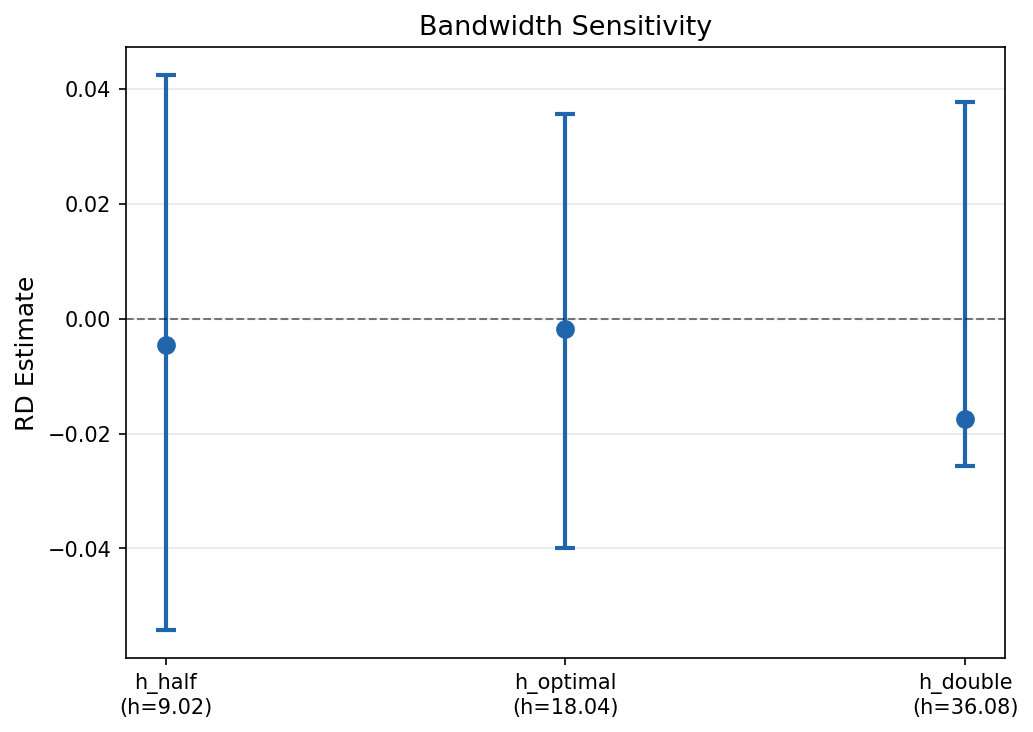
\includegraphics[width=0.9\textwidth]{figures/figure_2_bandwidth_sensitivity.png}
\caption{Bandwidth Sensitivity (Full ENAHO Sample). Point estimates
and 95\% confidence intervals for \texttt{TIENE\_BILLETERA} across
bandwidth choices from $h^*/2$ to $2h^*$. Estimates are near zero across
the range and confidence intervals consistently cover zero.}
\label{fig:bw_sensitivity}
\end{figure}

\begin{figure}[H]
\centering
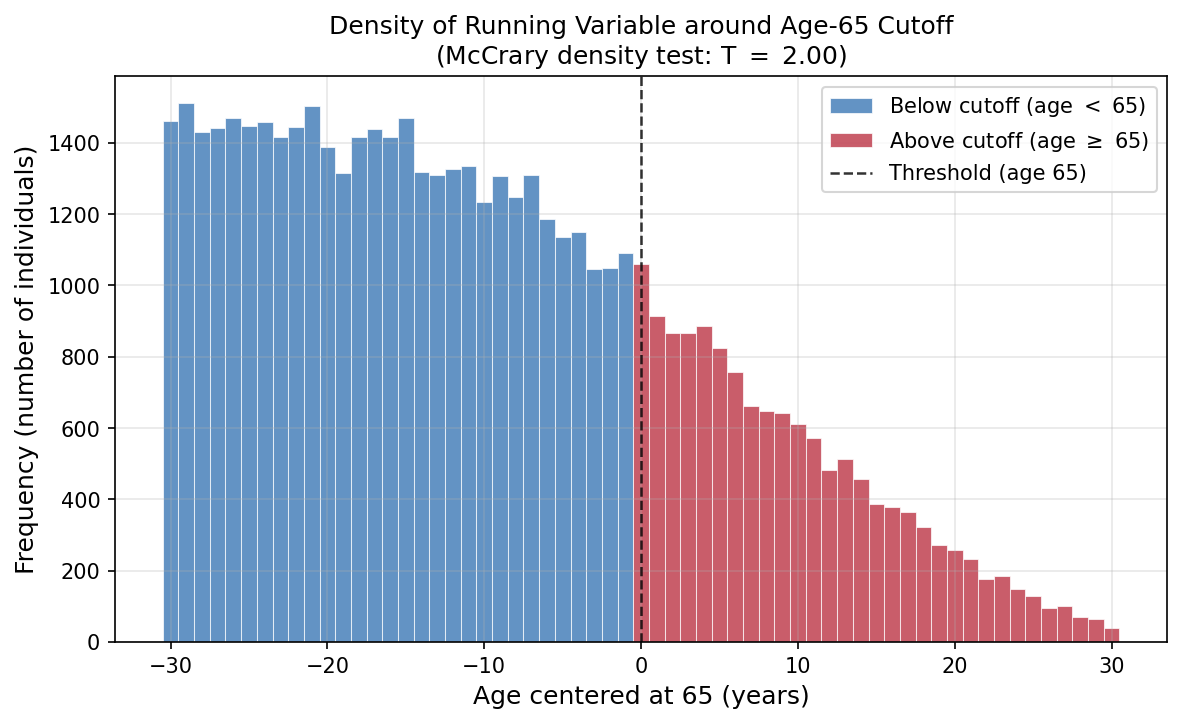
\includegraphics[width=0.9\textwidth]{figures/figure_mccrary_density.png}
\caption{Density of the Running Variable around the Age-65 Cutoff
(Full ENAHO Sample). Integer-age mass points are visible (a feature of
self-reported age in completed years), but there is no bunching specifically
at age~65 relative to adjacent integer ages, supporting the no-manipulation
assumption.}
\label{fig:mccrary}
\end{figure}

\begin{figure}[H]
\centering
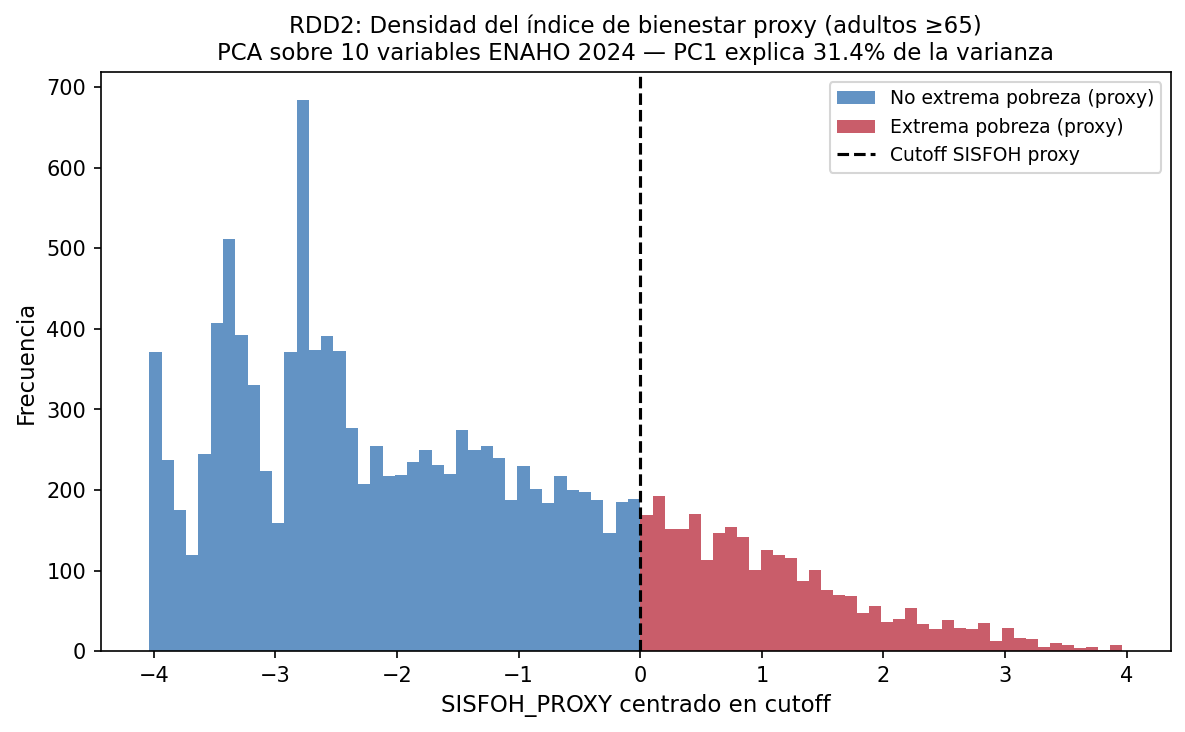
\includegraphics[width=0.9\textwidth]{figures/figure_rdd2_density.png}
\caption{RDD2: Density of the SISFOH Proxy Welfare Index around the
Estimated Poverty Threshold (Adults aged $\ge 65$). Blue bars indicate
individuals classified as non-extreme-poor (proxy below cutoff); red bars
indicate extreme-poor (proxy above cutoff). The absence of precise bunching
at the estimated threshold supports the continuity assumption for the
welfare-index design.}
\label{fig:rdd2_density}
\end{figure}


% =================================================================
% Appendix
% =================================================================
\clearpage
\appendix

\section{Extreme-Poor Subsample: Descriptive Estimates}
\label{sec:appendix_ep}

Table~\ref{tab:A1_ep} reports the \texttt{EP\_descriptivo} estimates from
the extreme-poor subsample (df\_main, $N=6{,}717$). These estimates are the
baseline RDD results within the SISFOH extreme-poor subgroup and
\textbf{should be interpreted as the subgroup-specific ITT for the
program's statutory target population}. Power is limited due to the small
share ($\approx\!5\%$) of extreme-poor respondents near the age-65 cutoff.
The positive estimate ($+0.027$ for \texttt{TIENE\_BILLETERA}) contrasts
with the near-zero full-sample result, illustrating the dilution bias
quantified in Section~\ref{sec:dilution}.

\begin{table}[H]
\centering
\caption{Extreme-Poor Subsample: Baseline RDD Estimates (Appendix)}
\label{tab:A1_ep}
\begin{threeparttable}
\begin{tabular}{l cc}
\toprule
\multicolumn{3}{c}{\textit{Appendix: Extreme-Poor Subsample (Descriptive)}} \\
\midrule
  & TIENE\_BILLETERA & USA\_BILLETERA \\
\midrule
\addlinespace
\multicolumn{3}{l}{\textit{EP\_descriptivo}} \\
  Estimate & 0.0272 & 0.0000 \\
  SE (robust) & (0.0218) & (0.0008) \\
  95\% CI & [-0.0139, 0.0717] & [-0.0030, -0.0001] \\
  N / BW & 1{,}144 / 13.95 & 663 / 7.64 \\
  Method & rdrobust & rdrobust \\
\bottomrule
\end{tabular}
\begin{tablenotes}
\small
\item \textit{Notes:} These estimates describe the RDD estimates within the extreme-poor subsample (POBREZA$=1$) for reference. Power is limited due to the small share of extreme-poor respondents ($\approx5\%$) near the age-65 cutoff.
\end{tablenotes}
\end{threeparttable}
\end{table}


% =================================================================
% References
% =================================================================
\clearpage

\begin{thebibliography}{99}

\bibitem[Aizenman et~al.(2022)]{aizenman2022}
Aizenman, J., Jinjarak, Y., and Park, D. (2022).
Cash-Transfer Eligibility Thresholds and Digital Savings: Evidence from
Latin America.
\textit{Journal of Development Economics}, 158:102934.

\bibitem[Angrist and Pischke(2009)]{angrist2009}
Angrist, J.~D. and Pischke, J.-S. (2009).
\textit{Mostly Harmless Econometrics: An Empiricist's Companion}.
Princeton University Press, Princeton, NJ.

\bibitem[Ardington et~al.(2016)]{ardington2016}
Ardington, C., Case, A., and Hosegood, V. (2016).
Labor Supply Responses to Large Social Transfers: Longitudinal Evidence
from South Africa.
\textit{American Economic Journal: Applied Economics}, 8(1):22--48.

\bibitem[Bachas et~al.(2018)]{bachas2018}
Bachas, P., Gertler, P., Higgins, S., and Seira, E. (2018).
Digital Financial Services Go a Long Way: Transaction Costs and Financial
Inclusion.
\textit{AEA Papers and Proceedings}, 108:444--448.

\bibitem[Banerjee et~al.(2020)]{banerjee2020}
Banerjee, A., Niehaus, P., and Suri, T. (2020).
Universal Basic Income in the Developing World.
\textit{Annual Review of Economics}, 11:959--983.

\bibitem[Bando et~al.(2020)]{bando2020}
Bando, R., Galiani, S., and Gertler, P. (2020).
The Effects of Non-Contributory Pensions on Material and Subjective
Well-Being: Evidence from a Randomized Control Trial.
\textit{Economic Development and Cultural Change}, 68(4):1233--1255.

\bibitem[Battistin et~al.(2009)]{battistin2009}
Battistin, E., Brugiavini, A., Rettore, E., and Weber, G. (2009).
The Retirement Consumption Puzzle: Evidence from a Regression Discontinuity
Approach.
\textit{American Economic Review}, 99(5):2209--2226.

\bibitem[BCRP(2024)]{bcrp2024report}
Banco Central de Reserva del Per\'u (2024).
\textit{Reporte de Inclusi\'on Financiera y Medios de Pago Digitales, 2024}.
Lima: BCRP.

\bibitem[BIS(2024)]{bis2024}
Bank for International Settlements (2024).
Digital Payments and Financial Inclusion in Developing Economies.
\textit{BIS Working Papers}, No.~1200. Basel: BIS.

\bibitem[Bruhn and Love(2014)]{bruhn2014}
Bruhn, M. and Love, I. (2014).
The Real Impact of Improved Access to Finance: Evidence from Mexico.
\textit{Journal of Finance}, 69(3):1347--1376.

\bibitem[Calonico et~al.(2014)]{calonico2014}
Calonico, S., Cattaneo, M.~D., and Titiunik, R. (2014).
Robust Nonparametric Confidence Intervals for Regression-Discontinuity
Designs.
\textit{Econometrica}, 82(6):2295--2326.

\bibitem[Calonico et~al.(2019)]{calonico2019}
Calonico, S., Cattaneo, M.~D., Farrell, M.~H., and Titiunik, R. (2019).
Regression Discontinuity Designs Using Covariates.
\textit{Review of Economics and Statistics}, 101(3):442--451.

\bibitem[Card et~al.(2008)]{card2008}
Card, D., Dobkin, C., and Maestas, N. (2008).
The Impact of Nearly Universal Insurance Coverage on Health Care
Utilization: Evidence from Medicare.
\textit{American Economic Review}, 98(5):2242--2258.

\bibitem[Cattaneo et~al.(2018)]{cattaneo2018}
Cattaneo, M.~D., Jansson, M., and Ma, X. (2018).
Manipulation Testing Based on Density Discontinuity.
\textit{Stata Journal}, 18(1):234--261.

\bibitem[Galiani et~al.(2020)]{galiani2020}
Galiani, S., Gertler, P., Bando, R., and Higgins, S. (2020).
Effect of the Digitization of Cash Transfers on Saving Behavior in
Argentina.
\textit{World Bank Economic Review}, 34(Supplement):S57--S69.

\bibitem[Jack and Suri(2014)]{jack2014}
Jack, W. and Suri, T. (2014).
Risk Sharing and Transactions Costs: Evidence from Kenya's Mobile Money
Revolution.
\textit{American Economic Review}, 104(1):183--223.

\bibitem[Muralidharan et~al.(2016)]{muralidharan2016}
Muralidharan, K., Niehaus, P., and Sukhtankar, S. (2016).
Building State Capacity: Evidence from Biometric Smartcards in India.
\textit{American Economic Review}, 106(10):2895--2929.

\bibitem[Suhrcke et~al.(2024)]{suhrcke2024}
Suhrcke, M., Cecchini, S., and Andr\'es, A.~R. (2024).
Regional Infrastructure and the Financial Inclusion Effects of Social
Transfers in Latin America.
\textit{Journal of Development Studies}, 60(3):415--438.

\bibitem[Suri(2017)]{suri2017}
Suri, T. (2017).
Mobile Money.
\textit{Annual Review of Economics}, 9:497--520.

\end{thebibliography}

\end{document}
